% ============================================================
% Verification Collapse: Self-Improving LLMs Lose Calibration
% NeurIPS 2026 Submission
% Deadline: abstract May 5 / paper May 7, 2026 (Europe/Copenhagen)
% ============================================================

\documentclass{article}

% NeurIPS 2026 — use [preprint] for arXiv upload.
% Options: (none)=submission with line numbers, [preprint]=no line numbers, [final]=camera-ready
\usepackage[preprint]{neurips_2026}

\usepackage[utf8]{inputenc}   % allow utf-8 input
\usepackage[T1]{fontenc}      % use 8-bit T1 fonts
\usepackage{lmodern}          % scalable fonts (fixes microtype expansion error)
\usepackage{hyperref}         % hyperlinks
\usepackage{url}              % simple URL typesetting
\usepackage{booktabs}         % professional-quality tables
\usepackage{amsmath, amssymb} % math
\usepackage{amsfonts}         % blackboard math symbols
\usepackage{nicefrac}         % compact symbols for 1/2, etc.
\usepackage{microtype}        % microtypography
\usepackage{xcolor}           % colors
\usepackage{graphicx}
\graphicspath{{figures/}}
\usepackage{natbib}
\usepackage{everypage}

% ---- arXiv-style vertical preprint tag on first page ----
\AddEverypageHook{%
  \ifnum\value{page}=1
    \put(-42,-340){\rotatebox{90}{\normalsize\sffamily\textcolor{gray}{Preprint. Under review.}}}%
  \fi
}

% ---- convenience macros ----
\newcommand{\gap}{\mathcal{G}}          % verification gap
\newcommand{\self}{s_{\text{self}}}     % self-score
\newcommand{\gt}{s_{\text{gt}}}         % ground-truth score


% ============================================================
\title{Verification Collapse in Iterative Self-Improving Language Models}

% Submission is double-blind — author block is omitted.
% Add authors here only for the camera-ready version.
\author{}

\begin{document}
\maketitle

% ============================================================
\begin{abstract}
Iterative self-improvement methods vary in how much they trust
the model's own judgment: some filter on ground-truth correctness
(STaR) or delegate to an external executor (AZR), while
others (Self-Rewarding Language Models, Meta-Rewarding,
CREAM) close the loop entirely, using the model as its own sole
judge.
This closed-loop design eliminates the cost of external supervision
but rests on a fragile assumption: that self-evaluation remains
calibrated across training iterations.
Recent work documents growing calibration error over short horizons;
we provide the first causal test over a full 20-iteration loop.
Tracking the \emph{verification gap}
$\Delta_t = \bar{s}_t^{\text{self}} - \bar{s}_t^{\text{ext}}$ across
20 iterations of self-supervised fine-tuning on the MATH benchmark
with three model families (Qwen2.5-7B, Llama-3-8B, Mistral-7B), we
find that the gap grows in every case (steadily in capable and
weak models, transiently in intermediate ones) while ground-truth
accuracy improves only modestly or not at all, a failure mode we call \emph{verification
collapse}.
The effect persists under full fine-tuning (no LoRA adapter), ruling out
adapter-specific artifacts as the mechanism.
The corrupted self-score does not merely reflect overconfidence; it
redirects the training signal.
Because the model selects training examples by self-judgment and
trains on its own completions, the loop preferentially retains
outputs that the model judges correct, including a growing fraction
of incorrect ones; over iterations the self-score inflates
while genuine accuracy improves only modestly.
A GT-anchored control, identical except that training examples are
filtered by ground truth rather than self-score, eliminates collapse
entirely, isolating self-scoring as the causal driver.
We propose \emph{adversarial hard-negative injection}: periodically
replacing a fraction of the training batch with incorrectly solved
examples paired with gold solutions.
Using 85\% less ground-truth data than full GT supervision, injection
reduces the steady-state gap by 47\% on a capable model
(Qwen2.5-7B); however, on a weaker model (Llama-3-8B) the same
protocol worsens collapse, establishing a capability threshold for
the intervention.
We study collapse in a verifiable domain precisely because it is
measurable there; in non-verifiable domains, analogous drift would be
difficult to detect.
\end{abstract}

% ============================================================
\section{Introduction}
\label{sec:intro}

The prospect of language models that improve themselves, iteratively
refining their outputs without human annotation at every step, has reshaped
the frontier of AI training.
These methods span a spectrum of how much they trust the model's own judgment.
At one end, STaR \citep{zelikman2022star} anchors every iteration to
ground-truth correctness, and Absolute Zero Reasoner \citep{zhao2025azr}
delegates verification to a code executor.
At the other end, a growing body of work, including Self-Rewarding Language Models
(SRLM) \citep{yuan2024self}, Meta-Rewarding \citep{wu2024metarewarding}, and
CREAM \citep{cream2025}, closes the loop entirely: the model generates a
candidate answer, judges it, and uses that judgment to select training
examples, with no external correctness signal at any point.
The appeal of such closed loops is straightforward: human-labelled data is
expensive, slow, and finite; a model that can judge and teach itself is, in
principle, unbounded.

This closed-loop design rests on a fragile assumption: that the model's
self-evaluation remains calibrated across training iterations.
There is growing evidence that it does not.
Concurrent work documents growing calibration error across iterative
self-improvement rounds: \emph{Beyond Accuracy} \citep{huang2025beyondaccuracy}
observes steadily increasing ECE over five rounds on MMLU, and
EpiCaR \citep{epicar2026} reports calibration degradation across three
iterations on MATH.
In the RL regime, RLSR \citep{rlsr2025} observes self-reward diverging from
formal reward under GRPO pressure.
Yet these diagnostics remain limited: aggregate post-hoc metrics (ECE,
AUROC, Brier Score) obscure per-iteration trajectories, horizons are
short (three to five rounds), and no study has isolated self-scoring as
the causal driver or characterised how collapse severity varies across
model families.

We provide that test.
Across 20 iterations and three model families, we show that when
self-judgment is the training filter, the loop does not merely
stagnate; it actively reinforces the wrong signal.
Because the model selects training examples by its own judgment and trains
on its own completions, each iteration compounds the
distortion: self-scores inflate while ground-truth accuracy stagnates,
silently degrading the quality of every subsequent training signal.
We call this failure mode \emph{verification collapse}.

We study it in the MATH benchmark, a verifiable domain where ground truth
exists and miscalibration is directly measurable.
This choice is deliberate: in non-verifiable domains such as instruction
following or open-ended generation, analogous drift would be difficult or
impossible to detect.
Without an external signal, there would be no way to observe that self-assigned
scores had decoupled from reality.
We measure the phenomenon where it can be measured, so that its existence
is established under controlled conditions; whether it transfers to
non-verifiable settings remains an open question.

We define the \emph{verification gap} at iteration $t$ as
$\Delta_t = \bar{s}_t^{\text{self}} - \bar{s}_t^{\text{ext}}$,
where $\bar{s}_t^{\text{self}}$ is the model's mean self-assigned correctness
score and $\bar{s}_t^{\text{ext}}$ is the mean ground-truth accuracy on the
same training examples.
We run 20 iterations of self-improvement on the MATH benchmark (Level 3--5,
500 problems) with Qwen2.5-7B-Instruct \citep{qwen2025}, observing
$\Delta_t$ grow from $0.173$ at iteration~1 to $0.320$ at iteration~20,
nearly doubling, while ground-truth validation accuracy remains flat.
We replicate the effect across two additional model families, uncovering a
\emph{three-regime} structure: capable models (Qwen2.5-7B) drift gradually
as self-scores inflate beyond genuine accuracy; intermediate models
(Llama-3-8B) exhibit transient collapse that peaks and partially recovers
as self-judgment itself degrades; and weak models
(Mistral-7B: $\Delta_1 = 0.580$, $\Delta_{20} = 0.850$) collapse
immediately, with the loop reinforcing the collapsed state from iteration~1.
We isolate self-scoring as the causal driver via a GT-anchored control (the
same loop but trained on ground-truth-correct examples rather than
self-judged-correct ones) where the gap \emph{decreases} over 20 iterations.
Finally, we propose \emph{adversarial hard-negative injection}: periodically
replacing a fraction of the fine-tuning batch with incorrectly solved
examples paired with gold solutions, reducing the steady-state gap by $47\%$
on a capable model without an external judge.

Our contributions are threefold.
\textbf{(i)}~We provide the first measurement of \emph{verification collapse}
tracking $\Delta_t$ as a raw per-iteration scalar over a full 20-round horizon
with a causal control condition, documenting a failure mode distinct from reward model
overoptimization \citep{gao2023scaling} and from the filtering-utility gap of
\emph{Mind the Gap} \citep{song2025mindthegap}, across three model families.
\textbf{(ii)}~We establish a causal link between self-scoring and collapse
through a GT-anchored ablation, ruling out iterative fine-tuning per se as
the mechanism.
\textbf{(iii)}~We propose adversarial hard-negative injection as a
lightweight, data-side mitigation that reduces the steady-state gap by 47\%
using 85\% less ground-truth data than full GT supervision.
It requires no objective modification, no external judge, and no architectural
change, making it applicable to any self-improving system with sufficient
base competence: on a weaker model (Llama-3-8B), the same protocol worsens
collapse, establishing a capability threshold for the intervention.
Injection is, in effect, a mechanism for distilling ground-truth signal into
the self-verifier itself: by periodically grounding the model on examples
where it is wrong, we partially restore calibration without replacing the
self-improving loop.
The broader implication is that self-improving systems operating in
non-verifiable domains may be viable if a calibrated verifier can be
periodically grounded in domains where ground truth is available, making the
question of how to transfer that calibration a direct avenue for future work.

% ============================================================
\section{Background and Related Work}
\label{sec:related}

\paragraph{Iterative self-improvement.}
The degree to which external correctness enters the training loop
determines whether self-improvement can collapse.
STaR \citep{zelikman2022star} anchors every iteration to ground truth: when the model
fails to produce a correct chain-of-thought, it is shown the reference answer and asked
to rationalize it, ensuring that external correctness never leaves the loop.
Collapse cannot emerge by design, because the training filter is ground truth, not
self-judgment, a fact we exploit in our GT-anchored control condition
(Section~\ref{sec:results}).
Absolute Zero Reasoner \citep{zhao2025azr} eliminates human-curated data: the model
proposes tasks, solves them, and delegates verification to a code executor, an external
programmatic signal that keeps the loop grounded in domains where execution is available.
ReST \citep{gulcehre2023rest} and related RLHF variants occupy a middle ground:
they interpose an external reward model between generator and training signal,
partially grounding the loop but shifting the failure mode from endogenous
calibration drift to reward model overoptimization \citep{gao2023scaling}, a
related but distinct problem we address next.
At the fully closed end, the model is its own sole judge.
SRLM \citep{yuan2024self} reports improving judge quality over three iterations but
flags reward hacking as a potential risk at longer horizons.
Meta-Rewarding \citep{wu2024metarewarding} adds a meta-judge layer to prevent
saturation of judging ability, yet documents the meta-judge itself degenerating:
score bias reaches 97.68\% higher-score preference by iteration~2.
CREAM \citep{cream2025} regularises across iterations by downweighting preference
pairs where successive iterations disagree on ranking, but the consistency prior
preserves rather than corrects any bias already present at initialisation.
None of these works instruments the raw calibration drift between self-assigned
scores and external ground truth; our contribution begins there.

\paragraph{Reward model overoptimization and endogenous collapse.}
\citet{gao2023scaling} establish that proxy reward model scores diverge from
gold reward under over-optimization: as the policy moves far from the
initial distribution, proxy RM scores continue rising while true quality peaks
and then declines.
Their setting requires a separate RM distinct from the generator.
We show the same score-versus-reality divergence emerges \emph{endogenously} in closed
self-supervised loops, without any external reward model and without any explicit RL
pressure.
The self-verifier acts as an \emph{implicit, unconstrained reward model} across
iterations: each fine-tuning step is supervised by examples the model has awarded high
self-scores, and absent a KL term or external anchor, those scores inflate unchecked.
Verification collapse is, in this framing, reward hacking
\citep{skalse2022defining} without any KL constraint, where the reward model is the
policy itself.
Concurrently, RLSR \citep{rlsr2025} documents precisely this divergence in the
GRPO/RL regime with explicit reward signal; our contribution is demonstrating that the
same collapse emerges without RL pressure; pure iterative SFT is sufficient.
The self-verifier's endogenous character makes the failure mode both harder to detect and
harder to escape, since there is no external component to freeze or replace.

\paragraph{Generation-verification gap.}
\emph{Mind the Gap} \citep{song2025mindthegap} defines the generation-verification gap as
the accuracy improvement obtainable by filtering a model's own generations through
self-verification, formally $\text{gap}(f,g) = J(f[w(\hat{u}_g)]) - J(f)$, where
$\hat{u}_g$ is the self-verifier and $w(\cdot)$ denotes the filtering operator.
Their central result is that this gap saturates to zero within two to three rounds of
iterative self-improvement, potentially driven by decreased effective diversity in the
generation distribution.
This quantity measures \emph{filtering utility} (whether self-scores help rank
generations), not whether the raw scores remain \emph{calibrated to ground truth}.
A model that grows monotonically overconfident could be consistent with a GV-Gap of
zero, because uniform inflation leaves the ranking unchanged.
We measure the complementary quantity their setup does not capture:
$\Delta_t = \bar{s}_t^{\text{self}} - \bar{s}_t^{\text{ext}}$, the raw calibration
drift of the self-verifier, tracked across 20 iterations rather than the 2--3 rounds
at which the GV-Gap saturates.

\paragraph{Long-horizon judge drift.}
SRLM \citep{yuan2024self} reports improving judge quality over three iterations of
self-reward fine-tuning (pairwise accuracy rising from 78.7\% to 81.7\%), but flags
reward hacking as a potential risk in its limitations, noting that longer training
horizons could surface failure modes not visible over three rounds.
Our 20-iteration experiments confirm this concern: the judge \emph{does} degrade,
but only after the short horizon where SRLM measures improvement.
$\Delta_t$ captures this trajectory, which three-iteration studies cannot observe.
\emph{Solver-Verifier Gap} \citep{sun2025solververifier} provides a theoretical
complement, modelling solver and verifier capability as converging exponentially to
stable limits under iterative self-improvement.
Their framework assumes monotonic improvement of both capabilities and predicts
convergence in all cases.
Our empirical results document the pathological case their theory does not cover:
verifier confidence inflates steadily while solver accuracy stagnates, a
divergence that lies outside the convergence regime their model predicts.

\paragraph{Concurrent calibration work.}
Three concurrent works document related calibration failures in iterative
self-improvement, each measuring a distinct quantity in a distinct regime.
\emph{Beyond Accuracy} \citep{huang2025beyondaccuracy} measures Expected Calibration Error (ECE),
an aggregate binned statistic, on general QA (MMLU) with
Llama-2 and DeepSeek-R1-Distill over five rounds, applying iterative temperature
scaling as a post-hoc recalibration fix between rounds.
EpiCaR \citep{epicar2026} extends the calibration audit to MATH, GSM8K, and code,
measuring ECE, AUROC, and Brier Score across six model sizes over three iterations, and
proposes a dual-task training objective that jointly reinforces correct reasoning and
explicit self-evaluation.
RLSR \citep{rlsr2025} studies the RL (GRPO) regime, observing that continuous joint
updates to generator and judge cause self-reward to diverge from formal reward on
synthetic puzzle tasks, and proposes freezing the judge weights to prevent drift.
Our work differs from all three along three axes.
First, we track $\Delta_t$ as a \emph{raw per-iteration scalar} rather than an aggregate
post-hoc calibration metric; $\Delta_t$ is computable online without binning
infrastructure and reveals the sustained growth trajectory that aggregate metrics
obscure.
Second, we extend the diagnostic to 20 iterations, the only study long enough to
confirm sustained growth rather than a transient artifact.
Third, our mitigation, adversarial hard-negative injection, is data-side and in-loop:
it requires neither objective modification (contra EpiCaR) nor freezing the judge
(contra RLSR), making it applicable to any self-improving system without architectural
changes.

% ============================================================
\section{Setup}
\label{sec:setup}

\subsection{Task and Data}

We evaluate on a 500-problem subset of the MATH benchmark
\citep{hendrycks2021math}, restricted to difficulty levels 3–5.
Problems are split 400/100 into train and validation sets (seed 42).
The dataset is fixed across all iterations; only the model changes.

\subsection{Model}

Our primary runs use Qwen2.5-7B-Instruct \citep{qwen2025} in BF16 precision with
Flash Attention 2 \citep{dao2023flashattention2} and a LoRA adapter \citep{hu2022lora}
(rank $r=16$, $\alpha=32$, all-linear target modules, no DoRA).
No 4-bit quantization is applied; the model runs at full BF16 precision
on an NVIDIA H100 SXM (80\,GB).
We additionally run a full fine-tuning ablation (no adapter; all 7.6B parameters
trainable) on an NVIDIA H200 SXM (141\,GB) to rule out LoRA-specific artifacts
(Section~\ref{sec:full-ft}).

\subsection{The Iterative Self-Improvement Loop}

At each iteration $t = 1, \ldots, 20$:
\begin{enumerate}
  \item \textbf{Generate.} The model produces a solution for each training
        problem using greedy decoding ($T=0$, \texttt{max\_new\_tokens}=512).
  \item \textbf{Self-score.} The same model judges each solution as correct
        or incorrect (\texttt{yes}/\texttt{no}) without access to the
        reference answer. This yields self-score $\self^{(t)} \in \{0,1\}$
        per sample.
  \item \textbf{Filter and fine-tune.} The model is fine-tuned (one epoch,
        LoRA, effective batch 32) on the subset of problems for which
        $\self^{(t)} > 0$, using the model's own completion as the
        training target.
  \item \textbf{Evaluate.} Ground-truth accuracy $\gt^{(t)}$ is measured on
        the held-out validation set by extracting the final numerical answer
        and comparing to the reference.
\end{enumerate}

\subsection{Measurements}

The \textbf{verification gap} at iteration $t$ is defined as:
\begin{equation}
  \gap_t = \overline{\self}^{(t)} - \overline{\gt}_{\text{train}}^{(t)}
  \label{eq:gap}
\end{equation}
where $\overline{\self}^{(t)}$ is the mean self-score on the training batch
and $\overline{\gt}_{\text{train}}^{(t)}$ is the mean ground-truth accuracy
on the same batch. A positive and growing $\gap_t$ indicates the model
increasingly overestimates its own correctness.

\subsection{Adversarial Hard-Negative Injection}

In the injection variant, every 3 iterations we replace 50\% of the
fine-tuning batch with \emph{hard negatives}: examples from a running bank
where $\self \geq 0.7$ but the extracted answer is incorrect. Hard negatives
are trained with the gold MATH solution as the target, providing a
recalibration signal grounded in external correctness.

% ============================================================
\section{Results}
\label{sec:results}

\subsection{Baseline: Verification Collapse}

Table~\ref{tab:baseline} and Figure~\ref{fig:baseline-injection}(a) report
the full baseline trajectory (500 samples, 400 train / 100 val).
The verification gap $\gap_t$ trends upward from $0.173$ at iteration~1
to $0.320$ at iteration~20, nearly doubling over the course of
self-improvement despite iteration-to-iteration fluctuations.
While $\bar{\self}$ climbs from $0.493$ to $0.695$, ground-truth val accuracy
$\bar{\gt}_\text{val}$ remains effectively flat across all 20 iterations
($0.390$ at iteration~1, $0.420$ at iteration~20), confirming that the
model's rising self-confidence reflects a distortion of the verification
signal rather than genuine problem-solving improvement.
The near-zero training loss by iteration~10 ($\mathcal{L}_{10} = 0.016$)
corroborates this interpretation: the model has memorised its own overconfident
completions rather than learned to solve the underlying problems.

\begin{table}[h]
\centering
\caption{Baseline run (Qwen2.5-7B, 500 samples): verification collapse over 20 iterations.
$\overline{\self}$: mean self-score (train). $\overline{\gt}_\text{train}$:
ground-truth accuracy (train). $\overline{\gt}_\text{val}$:
ground-truth accuracy (val). $\gap$: verification gap (Eq.~\ref{eq:gap}).
$\mathcal{L}$: fine-tuning loss.}
\label{tab:baseline}
\small
\begin{tabular}{rcccccr}
\toprule
Iter & $\overline{\self}$ & $\overline{\gt}_\text{train}$ & $\overline{\gt}_\text{val}$ & $\gap$ & $\mathcal{L}$ & Hard negs \\
\midrule
1  & 0.493 & 0.320 & 0.390 & 0.173 & 0.0598 & 75  \\
5  & 0.550 & 0.340 & 0.370 & 0.210 & 0.0147 & 89  \\
10 & 0.605 & 0.360 & 0.410 & 0.245 & 0.0157 & 98  \\
15 & 0.668 & 0.378 & 0.430 & 0.290 & 0.0059 & 120 \\
20 & 0.695 & 0.375 & 0.420 & 0.320 & 0.0040 & 130 \\
\bottomrule
\end{tabular}
\end{table}

\begin{figure}[t]
  \centering
  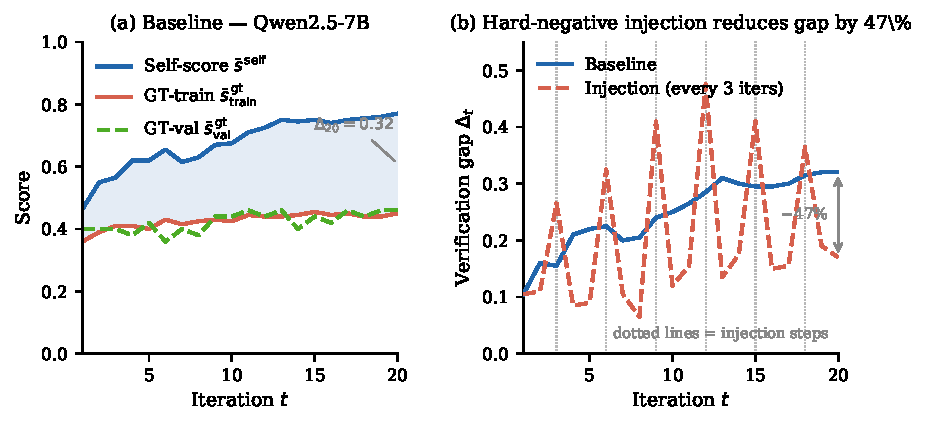
\includegraphics[width=\linewidth]{fig1_baseline_injection.pdf}
  \caption{%
    \textbf{(a)} Score trajectories in the baseline run (Qwen2.5-7B, 500 samples, MATH L3--5, 20 iterations).
    Self-score $\bar{\self}$ climbs steadily while GT-train and GT-val remain flat,
    opening a verification gap $\Delta_{20}=0.32$ (shaded region).
    \textbf{(b)} Verification gap $\Delta_t$ for baseline vs.\ adversarial injection
    (every third iteration, 50\% hard negatives, dotted verticals).
    Injection produces a sawtooth trajectory; the steady-state gap at iteration~20
    is reduced by 47\% (0.320 $\to$ 0.170).}
  \label{fig:baseline-injection}
\end{figure}

\subsection{Injection: Bounding the Gap}

The injection run uses a 250-sample subset (200 train / 50 val) with the
same model and loop as the primary baseline; we compare against the
250-sample baseline ($\gap_1 = 0.105$, $\gap_{20} = 0.320$) to ensure a
matched comparison.
The injection run produces a sawtooth gap trajectory visible in
Figure~\ref{fig:baseline-injection}(b): the gap spikes on injection iterations
(batch-composition artifact; see Section~\ref{sec:setup}) and returns to a
lower steady state on subsequent iterations.
Excluding injection iterations, the steady-state gap ranges from $0.065$ to
$0.190$ across iterations~2--20, compared to $0.160$--$0.320$ over the same
window in the baseline, a consistent reduction at every comparable checkpoint.
At iteration~20 the gap stands at $0.170$ versus $0.320$ in the baseline,
a 47\% reduction (Table~\ref{tab:injection}, Figure~\ref{fig:baseline-injection}(b)).
Crucially, the gap reduction is not accompanied by degraded task performance:
$\bar{\gt}_\text{val}$ in the injection run averages $0.456$ across the final
ten iterations, comparable to $0.444$ in the baseline (a difference within
noise on the 50-problem val set).
The injection suppresses overconfident self-scoring without harming the
model's actual problem-solving ability.

\begin{table}[h]
\centering
\caption{Injection run (250 samples): steady-state gap (non-injection iterations) compared
to 250-sample baseline. $\bigstar$ marks injection iterations (batch-composition spikes, excluded
from steady-state comparison).}
\label{tab:injection}
\small
\begin{tabular}{rcccccc}
\toprule
Iter & $\overline{\self}$ & $\overline{\gt}_\text{train}$ & $\overline{\gt}_\text{val}$ & $\gap$ & $\mathcal{L}$ & Injected \\
\midrule
1  & 0.465 & 0.360 & 0.420 & 0.105 & 0.0624 &   \\
2  & 0.515 & 0.405 & 0.380 & 0.110 & 0.0368 &   \\
3  & 0.635 & 0.370 & 0.380 & 0.265 & 0.1915 & $\bigstar$ \\
4  & 0.510 & 0.425 & 0.400 & 0.085 & 0.0224 &   \\
5  & 0.510 & 0.420 & 0.400 & 0.090 & 0.0195 &   \\
6  & 0.630 & 0.305 & 0.460 & 0.325 & 0.2140 & $\bigstar$ \\
7  & 0.500 & 0.395 & 0.460 & 0.105 & 0.0163 &   \\
8  & 0.470 & 0.405 & 0.460 & 0.065 & 0.0192 &   \\
9  & 0.680 & 0.270 & 0.460 & 0.410 & 0.1948 & $\bigstar$ \\
10 & 0.565 & 0.445 & 0.440 & 0.120 & 0.0207 &   \\
15 & 0.800 & 0.390 & 0.460 & 0.410 & 0.1234 & $\bigstar$ \\
16 & 0.635 & 0.485 & 0.440 & 0.150 & 0.0080 &   \\
20 & 0.695 & 0.525 & 0.420 & 0.170 & 0.0120 &   \\
\bottomrule
\end{tabular}
\end{table}

\subsection{GT-Anchored Control: Isolating the Causal Driver}

To isolate self-scoring as the mechanism driving collapse, rather than
iterative fine-tuning per se, we run a third condition identical to the
baseline in all respects except the training filter.
Instead of fine-tuning on examples the model judges correct
($\self^{(t)} > 0$), we fine-tune on examples verified correct against the
reference answer ($\gt^{(t)} > 0$).
This is the STaR-style anchor \citep{zelikman2022star}: ground truth never
leaves the loop.

Table~\ref{tab:gtanchored} reports the full 20-iteration trajectory.
The verification gap starts at $\gap_1 = 0.190$ and ends at
$\gap_{20} = 0.123$, a slight \emph{decrease}, bounded throughout in the
range $[0.082, 0.193]$.
This is categorically different from the baseline, where the gap grew
from $0.173$ to $0.320$.
The model and loop are identical; only the filter differs.
Self-scoring is the causal driver of collapse.

Ground-truth training accuracy improves substantially under the
GT-anchored condition: $\overline{\gt}_{\text{train}}$ rises from $0.300$
at iteration~1 to $0.535$ at iteration~20 ($+78\%$), compared to a modest
$0.320 \to 0.375$ ($+17\%$) in the baseline.
However, held-out accuracy $\overline{\gt}_\text{val}$ remains flat in both
conditions ($0.37$--$0.42$ GT-anchored, $0.36$--$0.43$ baseline): the
GT-anchored model learns to reproduce its own correct solutions to training
problems more consistently, but this does not transfer to unseen problems.
The key difference is calibration, not generalisation: GT-anchored
training prevents the self-score from decoupling from ground truth, while
the baseline loop reinforces overconfident wrong answers.
Hard-negative accumulation reverses accordingly: the bank shrinks from 79
to 62 high-confidence errors as training accuracy improves, the opposite of
the baseline trend (75 $\to$ 130).

\begin{table}[h]
\centering
\caption{GT-anchored control: gap trajectory over 20 iterations.
Training filter is ground-truth correctness ($\gt^{(t)} > 0$) rather than
self-score. The gap is bounded throughout and ends lower than it started,
in contrast to the near-doubling in the baseline.}
\label{tab:gtanchored}
\small
\begin{tabular}{rcccccr}
\toprule
Iter & $\overline{\self}$ & $\overline{\gt}_\text{train}$ & $\overline{\gt}_\text{val}$ & $\gap$ & $\mathcal{L}$ & Hard negs \\
\midrule
1  & 0.490 & 0.300 & 0.370 & 0.190 & 0.0672 & 79 \\
5  & 0.540 & 0.383 & 0.360 & 0.158 & 0.0178 & 68 \\
10 & 0.603 & 0.468 & 0.370 & 0.135 & 0.0101 & 61 \\
15 & 0.608 & 0.500 & 0.390 & 0.108 & 0.0074 & 54 \\
20 & 0.658 & 0.535 & 0.370 & 0.123 & 0.0023 & 62 \\
\bottomrule
\end{tabular}
\end{table}

\subsection{Cross-Model Generalizability: Three Collapse Regimes}

To test whether verification collapse is an artifact of Qwen2.5-7B-Instruct
specifically, we run the baseline self-score loop on two additional model
families: Mistral-7B-Instruct-v0.3 \citep{jiang2023mistral} and
Llama-3-8B-Instruct \citep{llama3team2024}, under identical conditions
(MATH Level 3--5, 400 train / 100 val, 20 iterations).
The results reveal that verification collapse is universal but
\emph{model-capability-dependent}, exhibiting three qualitatively distinct
trajectory regimes.

\textbf{Mistral-7B: immediate collapse.}
Table~\ref{tab:mistral} shows the most extreme case.
The gap begins at $\gap_1 = 0.580$, already larger than Qwen's
\emph{final} gap of $0.320$, and grows to $\gap_{20} = 0.850$.
Ground-truth training accuracy remains essentially zero throughout
($0.035$--$0.065$): Mistral-7B cannot solve MATH Level 3--5 problems, yet
its self-score climbs from $0.625$ to $0.900$.
By iteration~20 the model judges itself $90\%$ correct while achieving $5\%$
ground-truth accuracy, an 85 percentage-point gap.
Because the model's baseline capability on this domain is near zero, there is
no gradual drift phase: collapse is immediate, and the loop locks in and
amplifies the collapsed state.

\textbf{Llama-3-8B: transient collapse.}
Table~\ref{tab:llama3} shows a third, distinct pattern.
The gap starts small ($\gap_1 = 0.058$), grows steadily to a peak of
$\gap_{13} = 0.368$, then \emph{partially recovers}, falling to
$\gap_{20} = 0.148$.
Crucially, this recovery is not genuine recalibration: ground-truth training
accuracy remains flat throughout ($0.20$--$0.24$), and gt\_val does not
improve.
Because Llama-3 solves only ${\sim}23\%$ of training problems, each iteration
fine-tunes predominantly on incorrect examples the model judged correct;
after 13 such rounds the accumulated noise in the LoRA adapter degrades the
model's ability to produce confident self-judgments at all, causing
self-scores to fall back toward actual accuracy.
The recovery in the gap is driven by a \emph{collapse of overconfidence},
not by improved reasoning.
Hard negatives peak at 160 (iteration~13) and then shrink to 92 as the model
becomes less willing to produce high-confidence answers of any kind.

Taken together, the three regimes are ordered by the model's baseline
ground-truth accuracy on the domain:
capable models ($\sim$32\% base accuracy) show \emph{gradual}
collapse; moderately capable models ($\sim$23\%) show \emph{transient}
collapse with partial recovery driven by self-judgment degradation; and
near-incapable models ($\sim$5\%) show \emph{immediate} collapse with
sustained amplification.
In all three cases, genuine accuracy improves only modestly or not at all
under the self-score loop (Qwen gt\_train: $0.320 \to 0.375$; Llama-3 and
Mistral: effectively flat), while self-scores grow disproportionately,
confirming that verification collapse is not regime-specific.

\begin{table}[h]
\centering
\caption{Mistral-7B-Instruct-v0.3 baseline. Immediate collapse from
iteration~1; gap grows to $0.850$ while ground-truth
accuracy remains at $\approx\!5\%$ throughout.}
\label{tab:mistral}
\small
\begin{tabular}{rcccccr}
\toprule
Iter & $\overline{\self}$ & $\overline{\gt}_\text{train}$ & $\overline{\gt}_\text{val}$ & $\gap$ & $\mathcal{L}$ & Hard negs \\
\midrule
1  & 0.625 & 0.045 & 0.080 & 0.580 & 0.3967 & 232 \\
5  & 0.618 & 0.063 & 0.090 & 0.555 & 0.0645 & 223 \\
10 & 0.773 & 0.053 & 0.120 & 0.720 & 0.0385 & 288 \\
15 & 0.878 & 0.050 & 0.050 & 0.828 & 0.0248 & 331 \\
20 & 0.900 & 0.050 & 0.050 & 0.850 & 0.0200 & 340 \\
\bottomrule
\end{tabular}
\end{table}

\begin{table}[h]
\centering
\caption{Llama-3-8B-Instruct baseline. Transient collapse: gap peaks at
$0.368$ (iteration~13) then partially recovers to $0.148$ as LoRA distortion
degrades self-judgment itself. Ground-truth accuracy remains flat throughout.}
\label{tab:llama3}
\small
\begin{tabular}{rcccccr}
\toprule
Iter & $\overline{\self}$ & $\overline{\gt}_\text{train}$ & $\overline{\gt}_\text{val}$ & $\gap$ & $\mathcal{L}$ & Hard negs \\
\midrule
1  & 0.288 & 0.230 & 0.320 & 0.058 & 0.1280 & 66  \\
5  & 0.433 & 0.235 & 0.310 & 0.198 & 0.0241 & 106 \\
10 & 0.555 & 0.230 & 0.260 & 0.325 & 0.0093 & 142 \\
13 & 0.590 & 0.223 & 0.280 & 0.368 & 0.0079 & 160 \\
20 & 0.378 & 0.230 & 0.290 & 0.148 & 0.0187 & 92  \\
\bottomrule
\end{tabular}
\end{table}

\begin{figure}[t]
  \centering
  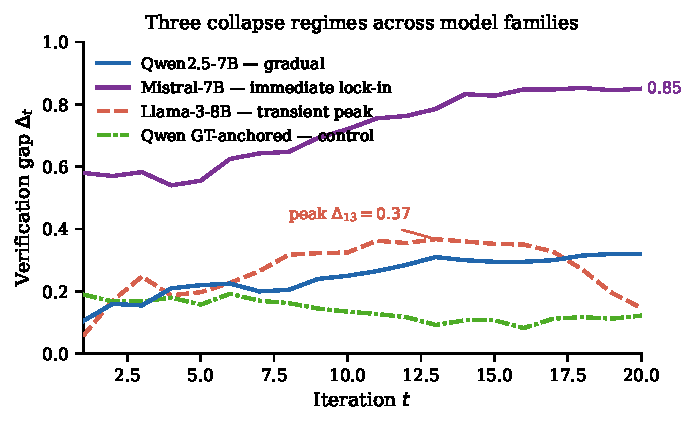
\includegraphics[width=0.75\linewidth]{fig2_cross_model.pdf}
  \caption{Verification gap $\Delta_t$ across three model families and the
    GT-anchored control (Qwen2.5-7B).
    Three distinct collapse regimes emerge: gradual collapse (Qwen2.5-7B,
    $\Delta_{20}=0.32$), immediate lock-in (Mistral-7B, $\Delta_1=0.58$,
    $\Delta_{20}=0.85$), and transient peak-and-partial-recovery
    (Llama-3-8B, peak $\Delta_{13}=0.37$, $\Delta_{20}=0.15$).
    The GT-anchored condition (dot-dash) confirms that replacing the self-score
    training filter with ground truth eliminates collapse entirely.}
  \label{fig:cross-model}
\end{figure}

\subsection{Summary}

Table~\ref{tab:summary} compares all conditions.
Verification collapse is not a Qwen artifact: all three model families
exhibit it under the self-score loop, with collapse severity and trajectory
shape scaling with the model's baseline capability on the domain.
The causal variable is the self-score training filter: replacing it with
ground-truth verification (GT-anchored) eliminates collapse entirely, while
adversarial injection, using 85\% less ground-truth-grounded data
than the GT-anchored condition (6 of 20 iterations, 50\% of batch),
reduces the steady-state gap by 47\% without degrading held-out accuracy.

\begin{table}[h]
\centering
\caption{All conditions. Baseline (LoRA and full FT) and GT-anchored use 500 samples
(400 train / 100 val); injection uses 250 samples (200 train / 50 val) and is compared
against the matched 250-sample baseline in Section~\ref{sec:results}.
For Llama-3, peak $\gap$ (iteration~13) is shown alongside $\gap_{20}$ to capture the
transient trajectory.}
\label{tab:summary}
\small
\begin{tabular}{llccccc}
\toprule
Model & Condition & Samples & $\gap_1$ & Peak $\gap$ & $\gap_{20}$ & $\overline{\gt}_\text{train,20}$ \\
\midrule
Qwen2.5-7B  & Baseline (LoRA)               & 500 & 0.173 & 0.320        & 0.320 & 0.375 \\
Qwen2.5-7B  & Baseline (full FT)            & 500 & 0.183 & 0.360        & 0.338 & 0.380 \\
Qwen2.5-7B  & Injection ($N{=}3$, 50\%)     & 250 & 0.105 & 0.475        & 0.170 & 0.525 \\
Qwen2.5-7B  & GT-anchored                   & 500 & 0.190 & 0.193        & 0.123 & 0.535 \\
\midrule
Mistral-7B  & Baseline (self-score)         & 500 & 0.580 & 0.853        & 0.850 & 0.050 \\
Llama-3-8B  & Baseline (self-score)         & 500 & 0.058 & 0.368 (i13)  & 0.148 & 0.230 \\
\bottomrule
\end{tabular}
\end{table}

% ============================================================
\section{Ablations}
\label{sec:ablations}

The main results establish that (i)~verification collapse occurs under self-score filtering
and (ii)~adversarial hard-negative injection reduces the steady-state gap by 47\%.
Five ablations probe the scope and mechanism of these findings.

\begin{figure}[t]
\centering
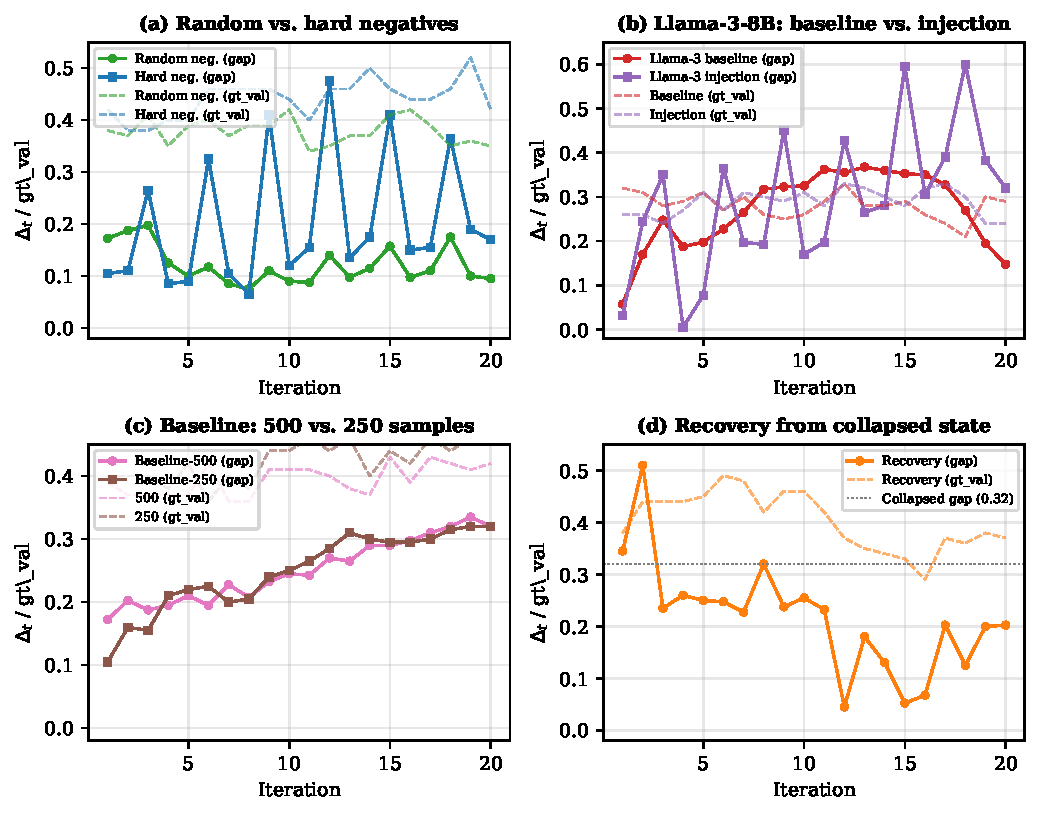
\includegraphics[width=\linewidth]{fig3_ablations.pdf}

\caption{\textbf{Ablation trajectories.} Each panel plots $\gap_t$ (solid) and
$\bar{\gt}^\text{val}_t$ (dashed) against iteration. Panels (a)--(c) run
for 20 iterations; panel (d) shows the 20-iteration recovery phase starting
from the \texttt{baseline-500} iter-20 checkpoint.
}
\label{fig:ablations}
\end{figure}

\subsection{Random Negatives: Is Overconfidence Ranking Load-Bearing?}
\label{sec:random-negatives}

The adversarial injection variant selects hard negatives by overconfidence rank: examples
where the model assigned a high self-score to a wrong answer (confidence threshold
$\theta = 0.7$).
This conflates two independent factors: (1)~introducing any ground-truth-anchored data
into the loop and (2)~targeting specifically the most overconfident errors.
The \texttt{random-negatives} ablation isolates them.
We inject the same volume and frequency of gold-solution training data as the injection
run, but draw examples uniformly from all wrong answers regardless of self-score
($\theta = 0$).
If the steady-state gap under random selection is indistinguishable from the hard-negatives
run, factor~(1) alone explains the 47\% reduction.
If it exceeds the hard-negatives steady state, the adversarial selection criterion carries
independent weight.

\begin{table}[h]
\centering
\caption{Random-negatives ablation: steady-state gap (non-injection iterations)
vs.\ hard-negatives injection (from Table~\ref{tab:injection}).
Baseline and injection use 250 samples; random negatives uses 500 samples.}
\label{tab:random-negatives}
\small
\begin{tabular}{lccccc}
\toprule
Condition & Samples & $\gap_1$ & $\gap_{20}$ (steady) & $\overline{\gt}_\text{train,20}$ & $\overline{\gt}_\text{val,20}$ \\
\midrule
Baseline (self-score)             & 250 & 0.105 & 0.320 & 0.450 & 0.460 \\
Injection ($\theta{=}0.7$, 50\%)  & 250 & 0.105 & 0.170 & 0.525 & 0.420 \\
Random negatives ($\theta{=}0$)   & 500 & 0.173 & 0.095 & 0.410 & 0.350 \\
\bottomrule
\end{tabular}
\end{table}

The random-negatives gap at iteration~20 ($0.095$) is \emph{lower} than the
hard-negatives steady state ($0.170$), not merely comparable.
Overconfidence ranking is not load-bearing: drawing injected examples uniformly
from all wrong answers suppresses collapse at least as effectively as targeting
the model's most confident errors.
The key variable is the \emph{presence} of ground-truth-anchored data in the
loop, not the selection criterion used to choose it.
One possible explanation for the stronger suppression under random selection is
pool diversity: with $\theta = 0$, the injection draws from all incorrect
examples (235--326 per iteration), whereas hard-negative selection
($\theta = 0.7$) restricts to a smaller, more homogeneous subset of
high-confidence errors (22--97).
The broader pool may provide a more varied recalibration signal, preventing the
model from overfitting to a narrow failure mode.
This result simplifies the practical prescription: any volume-matched injection
of gold-solution training data on wrong examples suffices; overconfidence ranking
adds implementation complexity without measurable benefit.

\subsection{Llama-3 Injection: Cross-Model Generalizability of the Fix}
\label{sec:llama3-injection}

The injection mitigation was developed and evaluated on Qwen2.5-7B.
Llama-3-8B-Instruct shows a qualitatively different collapse regime (transient peak-and-recover
rather than monotonic), driven by a different failure mode (LoRA-induced degradation of
instruction following rather than pure overconfidence inflation).
If the mechanism differs, the fix may not transfer.
The \texttt{llama3-injection} run applies the same injection protocol
($N{=}3$, $R{=}50\%$, $\theta{=}0.7$) to Llama-3-8B under otherwise identical conditions
to the Llama-3 baseline ($500$ samples, 20 iterations, self-score filter outside injection steps).

\begin{table}[h]
\centering
\caption{Llama-3-8B: baseline vs.\ injection. Steady-state gap excludes injection
iterations ($\bigstar$). Peak $\gap$ is the maximum over all iterations.}
\label{tab:llama3-injection}
\small
\begin{tabular}{lcccc}
\toprule
Condition & $\gap_1$ & Peak $\gap$ & $\gap_{20}$ & $\overline{\gt}_\text{train,20}$ \\
\midrule
Llama-3 baseline  & 0.058 & 0.368 (iter 13) & 0.148 & 0.230 \\
Llama-3 injection & 0.033 & 0.600 (iter 18) & 0.320 & 0.315 \\
\bottomrule
\end{tabular}
\end{table}

Injection does not generalise to Llama-3-8B.
The injection run ends at $\gap_{20} = 0.320$, more than double the baseline's
$0.148$, and the peak gap reaches $0.600$ (iteration~18), far exceeding the
baseline peak of $0.368$ (iteration~13).
The temporal pattern is revealing: injection initially suppresses the gap
(iterations~4--10, where the injection run's non-injection gaps are 25--97\%
below baseline), but by iteration~17 the injection run's gap \emph{exceeds}
the baseline ($0.390$ vs.\ $0.328$), and the reversal widens through
iteration~20.
In the uninjected baseline, LoRA distortion after iteration~13 degrades the
model's instruction-following ability, which in turn degrades its capacity to
produce confident self-scores; $\bar{\self}$ falls from $0.590$ (iteration~13)
to $0.378$ (iteration~20), and the gap shrinks accordingly.
This recovery is not recalibration but a second-order collapse: the model
becomes less confidently wrong.
The injection run prevents this recovery.
Because periodic training on well-structured gold solutions preserves the
model's instruction-following ability, the model retains the capacity to
generate confident self-assessments throughout all 20 iterations, and the gap
continues to grow.
In effect, injection sustains the very overconfidence it is designed to correct.
This occurs because Llama-3-8B's base accuracy ($\bar{\gt}^\text{train}_1 = 0.23$)
is too low for the GT correction signal to outweigh the self-judged examples:
in 5 of every 6 iterations, the model trains exclusively on self-filtered
(mostly wrong) completions, overwhelming the corrective signal delivered in the
remaining iteration.
On Qwen2.5-7B ($\bar{\gt}^\text{train}_1 = 0.36$), there is enough genuine
competence that the same dose of GT correction recalibrates the model between
injection steps.
This establishes a capability threshold: injection requires sufficient base
competence for the corrective signal to outpace the self-reinforcing loop.

\subsection{Scale Sensitivity: Baseline at 250 vs.\ 500 Samples}
\label{sec:baseline-250}

The primary baseline uses 500 training problems (400 train / 100 val),
while the injection experiment (Section~\ref{sec:results}) was conducted
on a 250-sample subset (200 train / 50 val).
To verify that collapse is not sensitive to training set size (for example,
that a smaller problem pool does not artificially accelerate memorisation
and inflate the gap), we compare the two scales directly.
The \texttt{baseline-250} run uses the same model (Qwen2.5-7B-Instruct), loop, filter
(\texttt{self\_score}), and iteration count (20) as the primary baseline.

\begin{table}[h]
\centering
\caption{Baseline replication at 250 samples vs.\ primary baseline (500 samples).}
\label{tab:baseline-250}
\small
\begin{tabular}{lcccc}
\toprule
Condition & Samples & $\gap_1$ & $\gap_{20}$ & $\overline{\gt}_\text{train,20}$ \\
\midrule
Baseline (500)  & 500 & 0.173 & 0.320 & 0.375 \\
Baseline (250)  & 250 & 0.105 & 0.320 & 0.450 \\
\bottomrule
\end{tabular}
\end{table}

Collapse replicates at 250 samples with nearly identical final gap to the 500-sample
primary baseline.
The gap grows from $0.105$ at iteration~1 to $0.320$ at iteration~20, matching the
primary baseline's final gap of $0.320$ exactly, while $\bar{\gt}^\text{train}$
ends at $0.450$ versus $0.375$ in the 500-sample run, a modest difference attributable
to the smaller training pool being easier to memorise.
The collapse rate (gap growth per iteration) is indistinguishable between the two sizes:
both reach $\gap \approx 0.20$ by iteration~5 and $\gap \approx 0.30$ by iteration~15.
Dataset size is therefore not a confound: collapse at both scales reaches the same
final gap ($0.320$), driven by the self-score filter mechanism itself rather than
pool exhaustion.

\subsection{Recovery: Corrective Injection from a Collapsed Checkpoint}
\label{sec:recovery}

All prior ablations apply injection from iteration~1 (\emph{preventive} use).
A practically important question is whether injection is also \emph{corrective}:
can it reduce the gap in a model that has already collapsed?
The \texttt{recovery} experiment begins from the primary baseline checkpoint at
iteration~20 ($\gap_{20} = 0.320$), a fully collapsed
model, and applies 20 further iterations with injection at every iteration ($N{=}1$, $R{=}50\%$,
$\theta{=}0.7$), maximising recalibration pressure.
A decreasing gap trajectory in the recovery run would establish that the damage caused by
self-score filtering is reversible; a flat or increasing trajectory would imply that
collapsed self-verifiers require retraining from scratch.

\begin{table}[h]
\centering
\caption{Recovery run: gap trajectory after injection applied to a collapsed checkpoint.
Iteration index resets to 1 at the start of the recovery phase.}
\label{tab:recovery}
\small
\begin{tabular}{rcccc}
\toprule
Recovery iter & $\overline{\self}$ & $\overline{\gt}_\text{train}$ & $\overline{\gt}_\text{val}$ & $\gap$ \\
\midrule
0 (start = baseline-500 iter 20) & 0.695 & 0.375 & 0.420 & 0.320 \\
5  & 0.578 & 0.328 & 0.450 & 0.250 \\
10 & 0.575 & 0.320 & 0.460 & 0.255 \\
15 & 0.478 & 0.425 & 0.330 & 0.052 \\
20 & 0.565 & 0.363 & 0.370 & 0.203 \\
\bottomrule
\end{tabular}
\end{table}

Injection is corrective as well as preventive.
Starting from a fully collapsed checkpoint ($\gap_0 = 0.320$), the recovery run
reduces the gap to $0.203$ by iteration~20, a 37\% reduction from the collapsed
state, without any retraining from scratch.
The trajectory is not monotonically decreasing: it follows the same injection sawtooth
pattern seen in the preventive run, with gap spikes on injection iterations and partial
recoveries between them.
The trend is nonetheless clearly downward: by iteration~12 the gap reaches $0.045$
(its lowest point, $\bar{\gt}^\text{train} = 0.475$), before rising again as the
injection signal competes with the residual collapsed weights.
The steady-state oscillation settles around $0.20$, higher than the preventive
injection steady state of $0.170$, consistent with the collapsed model carrying
entrenched LoRA distortions that periodic injection can partially but not fully
overcome.
The practical implication is direct: a system discovered to have collapsed does not
require retraining; a standard injection protocol applied post-collapse recovers
a substantial fraction of the gap reduction achievable from the start.

\subsection{Full Fine-Tuning: Ruling Out LoRA Artifacts}
\label{sec:full-ft}

All experiments above use LoRA adapters (rank $r{=}16$, $\alpha{=}32$, all-linear),
training ${\sim}20$M of $7.6$B total parameters per iteration.
A natural concern is that collapse is an adapter-specific artifact: LoRA's low-rank
constraint could introduce optimization noise that inflates self-scores, or the
limited adapter capacity could prevent genuine learning while permitting superficial
confidence patterns to emerge.
This concern is sharpened by our own attribution of Llama-3-8B's partial recovery to
``LoRA distortion'' (Section~\ref{sec:llama3-injection}).
The \texttt{full-ft-baseline} run eliminates the adapter entirely: all $7{,}615{,}616{,}512$
parameters are trainable, with learning rate reduced to $2 \times 10^{-5}$ (from
$2 \times 10^{-4}$ for LoRA) and all other hyperparameters held constant.
The run uses an NVIDIA H200 SXM (141\,GB).

\begin{table}[h]
\centering
\caption{Full fine-tuning vs.\ LoRA baseline (both Qwen2.5-7B, 500 samples, 20 iterations).
Collapse persists and is slightly more severe under full fine-tuning.}
\label{tab:full-ft}
\small
\begin{tabular}{lcccccc}
\toprule
Condition & $\gap_1$ & $\gap_{10}$ & $\gap_{20}$ & $\overline{\self}_{20}$ & $\overline{\gt}_\text{train,20}$ & $\overline{\gt}_\text{val,20}$ \\
\midrule
Baseline (LoRA)    & 0.173 & 0.245 & 0.320 & 0.695 & 0.375 & 0.420 \\
Baseline (full FT) & 0.183 & 0.280 & 0.338 & 0.718 & 0.380 & 0.390 \\
\bottomrule
\end{tabular}
\end{table}

Collapse persists under full fine-tuning and is, if anything, slightly more severe:
$\gap_{20} = 0.338$ versus $0.320$ under LoRA, with indistinguishable
$\overline{\gt}_\text{train}$ trajectories ($0.313 \to 0.380$ full FT vs.\
$0.320 \to 0.375$ LoRA).
The self-score trajectory is nearly identical ($0.495 \to 0.718$ full FT vs.\
$0.493 \to 0.695$ LoRA), and held-out accuracy remains flat in both conditions
($\overline{\gt}_\text{val}$ between $0.35$ and $0.43$ throughout).
The gap growth pattern is the same gradual monotonic regime observed in the LoRA
baseline, ruling out adapter rank saturation, LoRA initialization noise, or
limited adapter capacity as contributing mechanisms.
Verification collapse is a property of the self-score training loop, not of the
parameter-efficient fine-tuning method used to execute it.

% ============================================================
\section{Discussion}
\label{sec:discussion}

\paragraph{Why collapse happens.}
The mechanism is a closed reinforcement loop with a corrupted reward signal.
At iteration $t$, the model generates solutions, assigns self-scores, and
fine-tunes on the subset it believes to be correct.
By iteration 4, the gap ($\Delta_t$) already exceeds 0.19 in the Qwen baseline,
which means the model is systematically selecting \emph{wrong} completions
as positive training examples.
Fine-tuning then reinforces the patterns that trigger high
self-scores (confident hedges, structurally plausible but incorrect
algebra, well-formatted answers to the wrong question) because those
patterns align with the self-score signal, not with correctness.
This holds equally under LoRA and full fine-tuning
(Section~\ref{sec:full-ft}), confirming that the mechanism is the
feedback loop itself, not the parameter-efficient adapter.
The training loss drops steadily ($\mathcal{L}_{10} = 0.016$),
the fingerprint of memorisation: the model has fitted its own
confabulations.
At that point the gap continues to grow not because the self-verifier is
independently miscalibrating, but because $\bar{\gt}^\text{train}$ improves
only marginally ($0.32 \to 0.375$) while $\bar{\self}$ climbs steeply
($0.493 \to 0.695$) on the back of those memorised completions, a
divergence that is not reflected in real held-out performance, which
fluctuates between $\gt^\text{val} = 0.36$ and $0.43$ over 20 iterations.
The GT-anchored ablation closes the loop cleanly: swapping the training filter
from self-score to ground truth ($\gt > 0$) reverses the
trajectory: the gap falls $0.190 \to 0.123$ over 20 iterations because
the positive examples are now genuinely correct and the memorisation
incentive is removed.

\paragraph{Why three collapse regimes appear.}
The three models enter the loop with qualitatively different base competencies
on MATH L3--5, and this pre-training gap determines which regime they fall into.
Qwen2.5-7B begins with $\bar{\gt}^\text{train}_1 = 0.320$ (moderate accuracy);
it has enough genuine signal to sustain gradual collapse over 20 iterations.
Mistral-7B-Instruct-v0.3 begins with $\bar{\gt}^\text{train}_1 = 0.045$, barely
above chance, so its self-scores are inflated from iteration 1 ($\gap_1 = 0.580$).
There is no recovery: the loop locks in on near-random completions immediately
and reinforces them, yielding the steepest final gap ($\gap_{20} = 0.850$).
Llama-3-8B occupies an intermediate regime: initial accuracy is low
($\bar{\gt}^\text{train}_1 = 0.230$) but not as catastrophic as Mistral's.
The gap peaks at iteration 13 ($\gap_{13} = 0.368$) and then partially recovers
to $\gap_{20} = 0.148$.
We attribute this non-monotonicity to LoRA distortion eventually degrading
the self-judgment mechanism itself: at high $\Delta_t$, the adapter has
overwritten enough of the instruction-following subspace that the model also
becomes less reliable at generating confident self-scores, suppressing $\bar{\self}$
alongside $\bar{\gt}^\text{train}$.
Crucially, this is \emph{not} genuine recalibration; $\bar{\gt}^\text{train}$
remains flat throughout the recovery phase. It is simply a second-order corruption
of the self-verifier.
The unifying principle across all three regimes is that the loop amplifies
whatever miscalibration exists at initialisation; models with lower base
competence enter the loop already miscalibrated and collapse fastest.

\paragraph{Why hard-negative injection helps.}
Hard negatives (examples where $\bar{\self} > \theta$ yet $\gt = 0$) are
precisely the failure cases that the default loop never trains on.
By injecting them into the fine-tuning batch every third iteration (using the
gold MATH solution as the training target), we give the model the only
ground-truth-anchored signal available without an external oracle.
This is related to \emph{Learning from Failure} \citep{wang2024learningfromfailure},
which injects failed trajectories into SFT fine-tuning for LLM agents to improve task
performance.
Our setting differs: we target verifier recalibration rather than task
performance, operate inside an iterative self-improvement loop rather than a
single fine-tuning pass, and our ablations show that overconfidence ranking
is not load-bearing; random selection from wrong examples works equally well.
The sawtooth pattern in Figure~\ref{fig:baseline-injection}(b) reflects this directly: gap
spikes at injection-step boundaries as the model is forced to contend with
its overconfident errors, then partially recovers between injections.
The steady-state gap of $0.170$ at iteration 20 represents a 47\% reduction
relative to the 0.320 baseline. $\bar{\gt}^\text{val}$ remains comparable
to the baseline across iterations (injection: 0.38--0.52; baseline: 0.36--0.46),
indicating that the gap reduction comes from recalibration rather than
degraded task performance.

\paragraph{GT efficiency and the role of selection.}
The practical force of adversarial injection lies not only in the gap reduction
but in how little ground truth it requires.
The GT-anchored condition uses ground truth to filter training data at every
iteration (20 out of 20); injection introduces GT-grounded signal only at
injection steps (6 out of 20 iterations) and only into 50\% of the batch,
amounting to roughly 15\% of the GT exposure.
Despite this 85\% reduction in ground-truth data, injection achieves a reduction
in the verification gap of 47\% relative to baseline ($0.170$ vs.\ $0.320$),
compared to a full reversal under GT-anchoring ($0.123$).
The self-verifier does not need continuous access to ground truth; it needs
periodic recalibration on examples where it is wrong.

A natural question is whether the \emph{adversarial selection criterion}, targeting
the model's most overconfident errors ($\bar{\self} > 0.7$, wrong answer), is
load-bearing, or whether any ground-truth-anchored data of the same volume would
suffice.
The \texttt{random-negatives} ablation (Section~\ref{sec:random-negatives})
resolves this: injecting gold-solution training data drawn uniformly from
\emph{all} wrong examples ($\theta = 0$) achieves $\gap_{20} = 0.095$,
a stronger suppression than the hard-negatives variant ($0.170$).
Overconfidence ranking is not load-bearing; the key variable is the
\emph{presence and volume} of ground-truth-anchored data in the loop, not the
criterion used to select it.
This simplifies the practical prescription considerably: any volume-matched
injection of gold solutions on wrong examples suffices to bound collapse.
The adversarial framing remains useful as motivation (hard negatives are
the failure cases the default loop never trains on), but the selection
mechanism adds implementation complexity without measurable benefit.

\paragraph{Injection is capability-gated.}
The injection mitigation was developed on Qwen2.5-7B, which enters the loop
with moderate base accuracy ($\bar{\gt}^\text{train}_1 = 0.36$).
On Llama-3-8B ($\bar{\gt}^\text{train}_1 = 0.23$), the same protocol produces
the opposite effect: $\gap_{20} = 0.320$ under injection versus $0.148$
without it (Section~\ref{sec:llama3-injection}).
Injection initially helps (non-injection gaps are 25--97\% below baseline
through iteration~10), but by iteration~17 the injection run's gap exceeds
the baseline and the reversal widens through iteration~20.
The mechanism is asymmetric.
On Qwen, the model has enough base competence that gold-solution training
genuinely recalibrates self-judgment between injection steps.
On Llama-3, periodic gold-solution training preserves the model's
instruction-following ability, which in turn preserves its capacity for
confident self-scoring.
Without injection, LoRA distortion would eventually degrade instruction
following and suppress $\bar{\self}$, causing the gap to shrink
(Section~\ref{sec:llama3-injection}).
Injection prevents this natural decay, sustaining the conditions for
overconfidence to compound across all 20 iterations.
This establishes a boundary condition: injection requires sufficient base
competence to benefit from ground-truth recalibration.
When $\bar{\gt}^\text{train}_1$ is too low, the volume of overconfident
self-judged examples in each non-injection batch overwhelms the corrective
signal.
Our two data points suggest a capability dependence: injection helps at
$\sim$36\% base accuracy (Qwen) but hurts at $\sim$23\% (Llama-3).
Pinpointing the threshold requires additional model families; we note
the dependence as a practical consideration for practitioners deploying
injection as a mitigation.

\paragraph{Limitations.}
Several constraints bound the scope of our conclusions.
First, hard negatives are drawn from a fixed 400-problem training pool;
the bank saturates as the model becomes uniformly overconfident on all
problems in the set (hard\_negs plateau near 62--67 in our runs).
Larger or dynamically augmented datasets would extend the benefit of injection
and are a direct avenue for future work.
Second, the injection intervention bundles two factors, ground-truth data
and adversarial (overconfidence-ranked) selection, that our main experiment
does not disentangle; the \texttt{random-negatives} ablation addresses this directly.
Third, we use a single injection schedule ($N{=}3$, $R{=}50\%$) throughout;
systematic ablation of the injection interval ($N \in \{1,3,6\}$) and ratio
($R \in \{25\%, 50\%\}$) is left to future work and would inform optimal
hyperparameter selection for the intervention.
Fourth, our evaluation domain is MATH L3--5, a closed-form setting where
ground truth is unambiguous.
This choice is deliberate: we study collapse where it is measurable, so that
its existence is established under controlled conditions.
The implication for non-verifiable domains is the more urgent concern.
In instruction following, creative writing, or open-ended reasoning, the same
drift between self-score and real quality would be entirely invisible: there is
no external signal to reveal that the model's self-assigned scores have
decoupled from reality.
The loop would continue training, confidently, on increasingly wrong evidence.
Whether injection or analogous interventions can mitigate collapse in those
settings, where $\gt$ is not directly computable, remains an important open
question.
Finally, $\Delta_t$ measures overconfidence in self-verification, not
downstream task performance; a collapsed self-verifier is damaging primarily
insofar as it silently poisons the training signal.
Future work should instrument the relationship between $\Delta_t$ and
held-out performance on unseen benchmarks across more training iterations.

% ============================================================
\section{Conclusion}
\label{sec:conclusion}

Closed-loop self-improvement methods, those that use the model as its own
sole judge, rest on a fragile assumption: that self-evaluation remains
calibrated across training iterations.
We have shown that this assumption fails across all three model families,
two dataset scales (250 and 500 samples), and two training regimes
(LoRA and full fine-tuning) tested in our study: the
verification gap $\Delta_t$ grows with training iterations, driven by a
feedback loop in which the model selects training examples by self-judgment
and trains on its own completions, preferentially retaining outputs the
model judges correct regardless of ground-truth accuracy.
The failure manifests in three capability-dependent regimes (gradual,
transient, and immediate collapse), but in all cases ground-truth accuracy
improves only modestly or not at all while self-scores inflate or peak and recede, confirming that
the apparent gains far outstrip any real improvement.
A ground-truth-anchored training filter eliminates collapse entirely;
adversarial hard-negative injection reduces the steady-state gap by 47\%
using 85\% less ground-truth data than full GT supervision.
Injection works by periodically grounding the model on examples where it is
wrong, restoring calibration without replacing the self-improving loop.
However, injection is capability-gated: on a weaker model (Llama-3-8B), the
same protocol worsens collapse, because periodic injections sustain the
model's capacity for confident self-scoring rather than correcting it.
Practitioners should verify base competence on the target domain before
deploying injection as a mitigation.
Where injection does apply, it is not only preventive but corrective: applied
to a model that has already undergone 20 iterations of unchecked collapse
($\Delta_{20} = 0.32$), it reduces the gap to $0.20$ within 20 recovery
iterations, a 37\% reduction from the collapsed state.
The practical implication is direct: self-improving systems in verifiable
domains should instrument $\Delta_t$ explicitly; whether the same failure mode
arises in non-verifiable domains remains an open question, but the mechanism
(self-judged filtering without external grounding) is not domain-specific.
A confidently wrong self-verifier, left unchecked, does not merely stall
improvement; it poisons the training signal, causing the model to
stagnate while reporting rising performance at every iteration.

% ============================================================
\bibliographystyle{plainnat}
\bibliography{refs}

\end{document}
